
\chapter{Project I involved}
\begin{flushleft}
\label{ch:method}

We were a team of 11 members, 8 interns who are my classmates. And Masud bhai(CTO, Orbitax), Shaon bhai(Senior Software Engineer, Orbitax) And Plabon bhai(Associate Software Engineer, Orbitax) guided us thrugh our six months journey. It was a great experience working with them.


\section{Orbitax Connect}

Orbitax Connect is a mobile application developed for both Android and IOS. It gives a short glimpse of the total Orbitax platform to its user.
 As this project’s information was under NDA so we will talk about its basic overview.
  \begin{figure}[htbp]
\centerline{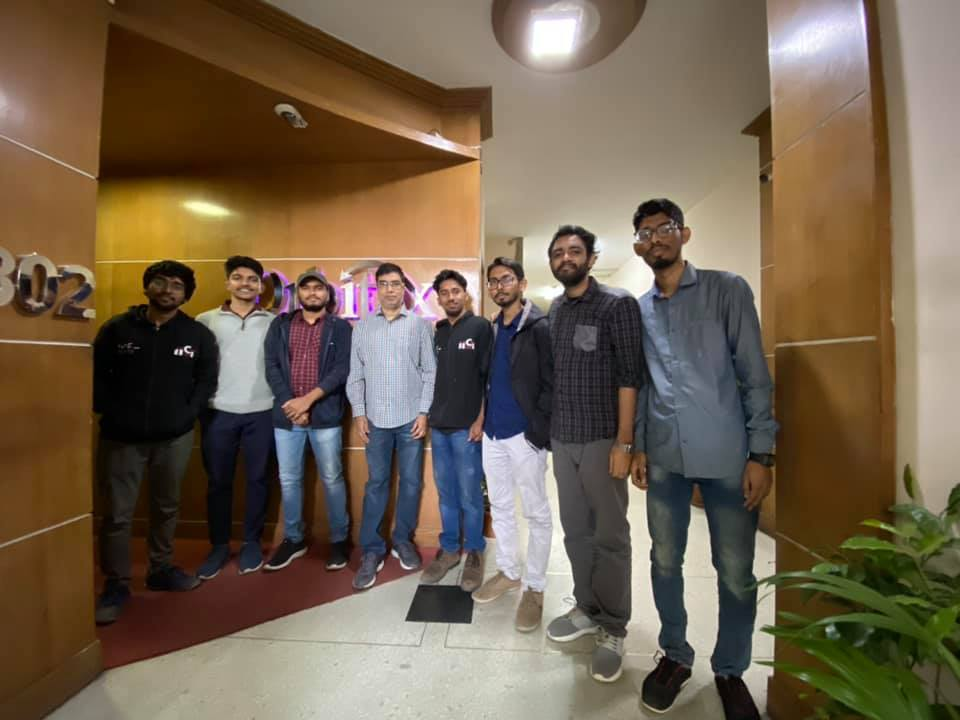
\includegraphics[scale=0.5]{Figures/interns.jpg}}
\caption{Intern team CTO,Orbitax}
\label{fig}
\end{figure}


\subsection{Overview}
Orbitax Connect is a pet project so its development process goes under the tag of a pet project. Being a pet project, orbitax does not compromise its quality, all of the development processes are strictly followed. When I was assigned to this project it’s just in its birth phase. 


\subsection{Team}
We all were assigned to the same project. But we were assigned as a pair. I was assigned with my batchmate Partha Pratim Paul for this project. We work on this project following the pair programming methodology. He was very helpful, hardworking and I got to learn so much from him. It was a pleasant experiance working with him. For some time I was also paired with Ahsan Aziz Ishan who is brilliant and dedicated about his responsibility and I enjoyed working with both of them.


\subsection{Technology}
What technology we used to complete this project are given below:

\begin{enumerate}
    \item Typescript
    \item NodeJs
    \item React
    \item React Native
    \item Redux
    \item Realm
    \item RxJs
    \item Lodash
    \item Jest
    \item Enzyme
    \item Git
    \item Various third party packages
 
\end{enumerate}


\subsection{Features I Was Worked}
I worked on  a library feature where recent tax news and changes reflect on a library system and a home screen where different types of feeds showed with Partha.\\ 

And I also worked in a contact feature where a client can chat,create group and do various things and in this feature I teamed up with Ishan. These were very important features of this project. For implementing these features, I have to learn graphql and implement my learning. I was successfully able to do my work. Besides graphql I used most of the technology mentioned above.


\subsection{Challenges}
The main challenge for me was that I just joined Orbitax and had little idea about industry projects. And I worked with most three people in varsity projects. So working with a big team was a bit challenging at first.  And I don’t have any knowledge of the Orbitax ecosystem. So at first, I have to struggle a little bit to make myself comfortable. After getting used to the ecosystem it’s being pretty comfortable.
The ecosystem of Orbitax is huge so you always find something to learn. The ecosystem is running the microservice architecture. And you will always find a service that does a certain task and it communicates with each other through message passing. As this was my first time with microservice work, so it takes a little bit of time to grasp it. It was a real challenge for me.
Then another thing was maintaining the coding structure. It seems difficult at first. But throughout the time I was comfortable with this. This was fun and the code was much easier to read and understand.
\end{flushleft}